% !TEX root = ../thesis.tex
Up until now, we did not specify the collision part of~\eqref{eq: lattice boltzmann equation}.
As stated in Section~\ref{sec: History of Lattice Boltzmann}, instead of calculating the collision, we can model the effect of multiple collisions, which is the shift towards a local equilibrium.
The different schemes distinguish themselves in the way they implement this shift.
In this section, the basic idea is elaborated in more detail and the most common methods are briefly presented.
\newlinedouble{}
Albeit not a physically sound reasoning, one can imagine a very big, frictionless billiard table to illustrate said shift.
Initially we roll all balls in the same direction but not perfectly parallel to the wall.
In the first few moments, those balls will go along in the same direction and the system will have a preferred direction and velocity, namely the direction and velocity we initiated.
After some time passed, the balls will have collided several times amongst themselves and the walls\footnote{The wall is only needed to make them collide amongst each other. For the result, the ball-ball collisions are the important ones, as they can change not only the direction but also the magnitude of their velocity. Alternatively one could also talk about the table being mirrored in every direction indefinitely which would have the same result, but that's a bit harder to imagine.} and they will have a plethora of different speeds and directions.
There's now no preferred direction and the distribution of speeds won't change anymore; the system is in an equilibrium.

Changing back to the continuous view, this equilibrium is known as the Maxwellian Distribution, which reads in two dimensions, c.f.~\cite{succi2001lattice}:
\begin{equation}
  \label{eq: maxwell distribution raw}
  f_{m, \rho, \vec{u}, T}^{\text{maxwell}}(\vec{\xi}) = \rho \frac{m}{2\pi k_B T} \exp \left( - \frac{m\norm{\vec{\xi}-\vec{u}}^2}{2 k_B T}\right)
\end{equation}
where the quantities are defined in Table~\ref{table: maxwell quantities}.
\begin{table} [h]
\centering
  \begin{tabular}{@{}ll@{}}
    \toprule
    Symbol & Quantity  \\
    \midrule
    $\vec{\xi}$  & Microscopic velocity  \\
    $\rho$ & Macroscopic density     \\
    $\vec{u}$    & Macroscopic velocity   \\
    $T$    & Temperature   \\
    $k_B$  & Boltzmann constant \\
    $m$    & Mass of the particles   \\
    \bottomrule
  \end{tabular}
\caption{Quantities occuring in the Maxwell distribution~\eqref{eq: maxwell distribution raw}}
\label{table: maxwell quantities}
\end{table}

One of the most popular Lattice-Boltzmann schemes, \gls{srt}, proceeds as following.
The $f_{ij}^{eq}$ are defined due to a yet unspecified discretization of~\eqref{eq: maxwell distribution raw} and the collision operator $\tilde{\Omega}$ of~\eqref{eq: define post collision} reads
\begin{equation*}
  \tilde{\Omega}(f_{ij}) \defined \omega \left(f_{ij}^{eq} - f_{ij}^{\circ}\right),
\end{equation*}
with an also unspecified `relaxation time' $\omega$.
This also gave the method its prominent name, as it uses only one parameter $\omega$ to relax all the~\glspl{pdf}.
Thus, equation~\eqref{eq: define post collision} reads now
\begin{equation}
  \label{eq: post collision discrete}
  f_{ij}^* = f_{ij}^{\circ} + \omega \left(f_{ij}^{eq} - f_{ij}^{\circ}\right) = (1-\omega)f_{ij}^{\circ} + \omega f_{ij}^{eq}.
\end{equation}
If $\omega\in[0,1]$ is chosen, this is exactly a linear interpolation, also called relaxation towards equilibrium, which is the modeled effect of the collision we motivated in the beginning.
This also explains the alternative name BGK-LBM of the \gls{srt}, after the inventors of the continuum analogue technique for the Boltzmann equation.
At this moment, though, we have no equation to fix $\omega$, but we will first deal with the problem of discretizing $f^{maxwell}$ into $f_{ij}^{eq}$.

The method of discretizing~\eqref{eq: maxwell distribution raw} used for \gls{srt} is due to a Taylor series expansion, yielding\footnote{The microscopic velocity is again delegated to the index $ij$, whereas $\rho$ and $\vec{u}$ are now parameters.
The factor $\frac{m}{k_B T}$ is constant and equal to the speed of sound $c_s$, more details in Section~\ref{sub: Equilibrium distribution for cumulants}.}
\begin{equation}
  \label{eq: equilibrium particle distributions}
  f_{ij}^{eq}(\rho,\vec{u}) = W_{ij}\rho
  \left[
    1
    + \frac{\vec{c}_{ij} \cdot \vec{u}}{c_s^2}
    + \frac{9}{2}\frac{{(\vec{c}_{ij} \cdot \vec{u})}^2}{c_s^4}
    - \frac{3}{2}\frac{\vec{u} \cdot \vec{u}}{c_s^2}
  \right],
\end{equation}
where $W_{ij}$ is a weighting factor depending on the chosen lattice, $c_s$ the speed of sound in the lattice and $\vec{c}_{ij}$ are the velocities defined in~\eqref{eq: definition of the velocities}.
As we can see here, $f^{eq}$ nonlinearly depends on all $f_{ij}$ via the macroscopic velocity and pressure.

When analyzing this method,~\cite[Section 5.2.3]{wolf2000lattice}, the kinematic viscosity $\nu$ (in lattice units) is actually calculated by
\begin{equation*}
  \nu = \frac{1}{3}\left(\frac{1}{\omega} - \frac{1}{2}\right).
\end{equation*}
Hence, to get to low viscosities, we need $\omega \rightarrow 2$ instead and thus to actually overrelax the \glspl{pdf} in~\eqref{eq: post collision discrete}.
The root of this seeming inconsistency is elucidated in~\cite[Section 4]{karlin2006elements} and stems from our discretization of~\eqref{eq: Boltzmann transport equation}.

On looking upon the nondimensionalized, incompressible Navier-Stokes equations,~\eqref{eq: navier stokes nondim}, we see that the \gls{re} is more telling than just the viscosity.
Consequently we will talk about the Reynolds number being very high instead of the viscosities being low.
Some typical values for \gls{re} are shown in Table~\ref{table: reynolds numbers}, stating the clear necessity of a numeric scheme that can handle a broad range of Reynolds numbers.
\def\stackalignment{l}
\setlength{\tabcolsep}{9pt}
\begin{table}
  \centering
  \begin{tabular}{l l rrr r}
    \toprule
    object & fluid & \multicolumn{4}{c}{values}    \\
    \cmidrule(lr){3-6}
           &       & $L [m]$  & $u_0[\frac{km}{h}]$ & $\nu[ \frac{m^2}{s}]$        & $Re$ \\
   \cmidrule(lr){1-6}
   Car   &
   \stackunder{Air}{\tiny{(ground level, $20^{\circ}C$)}}
   & $4$
   & $ 150 $
   & $1.478 \times 10^{-5} $
   & $1.41 \times 10^{7}$ \\
   Plane &
   \stackunder{Air}{\tiny{($10 km$ altitude, $-49.9^{\circ}C$)}}
   & $40$
   & $ 800 $
   & $3.526 \times 10^{-5} $
   & $2.52 \times 10^{8}$ \\
   \stackunder{Seabed}{\tiny{(porous media)}}
   & \stackunder{Water}{\tiny{($5^{\circ}C$)}}
   & $0.01$
   & $ 0.036 $
   & $1.519 \times 10^{-6} $
   & $6.58 \times 10^{1}$\\
   \bottomrule
  \end{tabular}
  \caption{Typical Reynolds numbers needed in simulations. Values for viscosity from~\cite{engToolbox,engToolbox2,wolframquery}}\label{table: reynolds numbers}.
\end{table}
Unfortunately, the SRT scheme develops serious instabilities for Reynolds numbers of some hundred or greater\footnote{This is not an exact value, but a rule of thumb. This value also depends on the other simulation settings}, as illustrated  by the checkerboard modes in Figure~\ref{fig: spurious modes SRT}. For higher Reynolds numbers, those instabilities take over, ruining the simulation. Albeit not a thorough analysis, this can be seen as a hint that \gls{lbm} may need further work to become a serious competitor in~\gls{cfd}.
\begin{figure}
\centering
\begin{subfigure}{.5\textwidth}
\label{fig: velocity SRT}
  \centering
  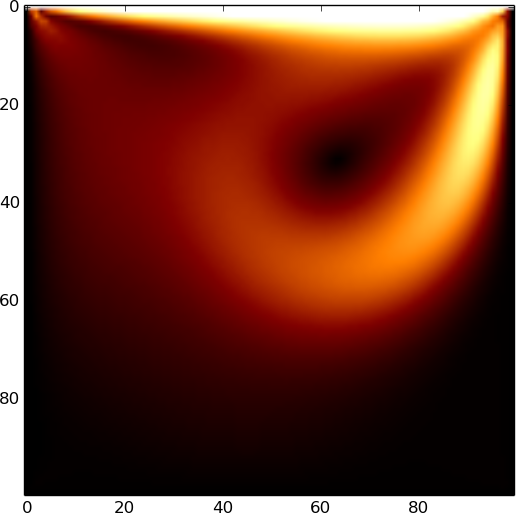
\includegraphics[width=0.8\linewidth]{../figures/ldc_re500_vel2_0019_trim.png} % chktex 11
  \caption{Velocity magnitude }
\end{subfigure}%
\begin{subfigure}{.5\textwidth}
\label{fig: density SRT}
  \centering
  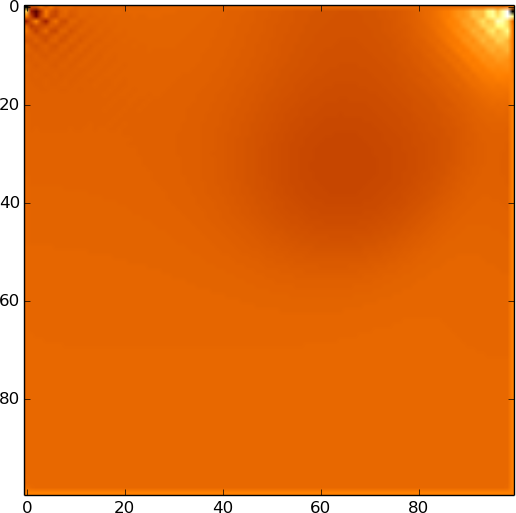
\includegraphics[width=0.8\linewidth]{../figures/ldc_re500_rho2_0019_trim.png} % chktex 11
  \caption{Density fluctuations}
\end{subfigure}
\caption[Lid driven cavity]{Simulation of a lid driven cavity\protect\footnotemark\ with SRT LBM at $Re=500$. Especially in the density field, we can see the checkerboard pattern of upcoming instabilities.}
\label{fig: spurious modes SRT}
\end{figure}
Intuitively, we can describe \gls{srt} as a scheme, where all non-conserved quantities which can be computed from the \glspl{pdf}, are relaxed at the same rate.
Hence we impose, that all events that happen in the fluid occur at the same rate, which is certainly not true.
\footnotetext{A lid driven cavity is a box filled with fluid, where all walls are fixed except the top one which moves with a prescribed velocity to the right.}

This was noticed soon after its publication and apparently the remedy was found by d'Humiéres,~\cite{d1994generalized}, who proposed to change from the space of particle distributions to the space of moments and relax linear combinations of those independently.
This was the birth of the \gls{mrt} schemes.
Unfortunately, even today there is no consent about how to choose all the relaxation parameters in an optimal way.
When chosen right, the accuracy and stability can improve greatly in contrast to SRT, allowing simulations of $Re$ in the low thousands, c.f.~\cite{d2002multiple}.
Still, this does not nearly cover the regions we see in Table~\ref{table: reynolds numbers}.

The source of these problems can be interpreted as the violation of \gls{galInv}, as deduced in~\cite{geier2006cascaded}. Consequently, the authors choose the space of central moments for the relaxation, as they are centered around the first moment, i.e.\ the velocity times density.
This method is capable of simulating \gls{re} way above the ones, \gls{mrt} is capable of and is used in industrial grade \gls{lbm} solvers, like \href{http://www.xflowcfd.com/technology/view/cfd}{xFlow}.

Regardlessly, we will introduce yet another set of characteristic variables in the next section and explain the physical reasoning behind choosing them.
